\subsection{Zener Diode:}

\begin{multicols}{2}
\begin{tasks}
\task {\bfseries\itshape First circuit:}
\begin{enumerate}
\item Zener Diode: 3.3 V
\item $R_{L}$ resistor: 33 $\Omega$.
\item $R_{lim}$ resistor: 82 $\Omega$.
\begin{figure}[H]
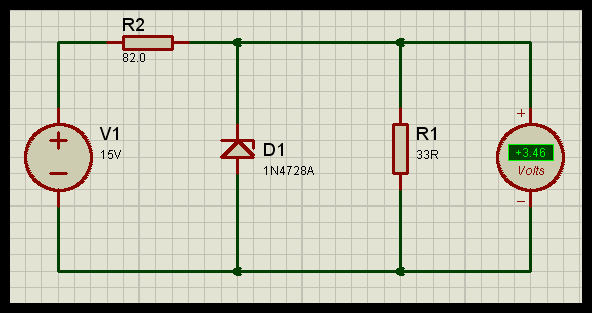
\includegraphics[scale=.405]{s2.png}
\centering \linebreak \linebreak Figure 4.1.0: 3.3 V Zener diode simulation.
\end{figure}
\end{enumerate}

\begin{center}
\begin{tabular}[.5cm]{ c c }
\toprule
Source Voltage & Voltage in $R_{L}$ \\
\midrule
3.0 V & 0.86 V \\
\cmidrule{1-2}
4.0 V & 1.15 V \\
\cmidrule{1-2}
5.0 V & 1.43 V \\
\cmidrule{1-2}
6.0 V & 1.72 V \\
\cmidrule{1-2}
7.0 V & 2.01 V \\
\cmidrule{1-2}
8.0 V & 2.30 V \\
\cmidrule{1-2}
9.0 V & 2.58 V \\
\cmidrule{1-2}
10.0 V & 2.87 V \\
\cmidrule{1-2}
11.0 V & 3.15 V \\
\cmidrule{1-2}
12.0 V & 3.27 V \\
\cmidrule{1-2}
13.0 V & 3.34 V \\
\cmidrule{1-2}
14.0 V & 3.40 V \\
\cmidrule{1-2}
15.0 V & 3.46 V \\
\bottomrule
\end{tabular}
\end{center} 

\task {\bfseries\itshape Second circuit:}
\begin{enumerate}
\item Zener Diode: 5.1 V
\item $R_{L}$ resistor: 49 $\Omega$.
\item $R_{lim}$ resistor: 56 $\Omega$.
\begin{figure}[H]
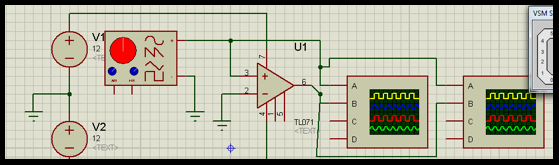
\includegraphics[scale=.4]{s1.png}
\centering \linebreak \linebreak Figure 4.1.1: 5.1 V Zener diode simulation.
\end{figure}
\end{enumerate}

\begin{center}
\begin{tabular}[.5cm]{ c c }
\toprule
Source Voltage & Voltage in $R_{L}$ \\
\midrule
3.0 V & 1.40 V \\
\cmidrule{1-2}
4.0 V & 1.87 V \\
\cmidrule{1-2}
5.0 V & 2.33 V \\
\cmidrule{1-2}
6.0 V & 2.80 V \\
\cmidrule{1-2}
7.0 V & 3.27 V \\
\cmidrule{1-2}
8.0 V & 3.73 V \\
\cmidrule{1-2}
9.0 V &  4.20 V \\
\cmidrule{1-2}
10.0 V & 4.63 V \\
\cmidrule{1-2}
11.0 V & 5.03 V \\
\cmidrule{1-2}
12.0 V & 5.16 V \\
\cmidrule{1-2}
13.0 V & 5.25 V \\
\cmidrule{1-2}
14.0 V & 5.33 V \\
\cmidrule{1-2}
15.0 V & 5.41 V \\
\bottomrule
\end{tabular}
\end{center}
\end{tasks}
\end{multicols}

\pagebreak

\begin{tasks}
\task {\bfseries\itshape Third circuit:}
\begin{enumerate}
\item Zener Diode: 9.1 V
\item $R_{L}$ resistor: 82 $\Omega$.
\item $R_{lim}$ resistor: 27 $\Omega$.
\begin{figure}[H]
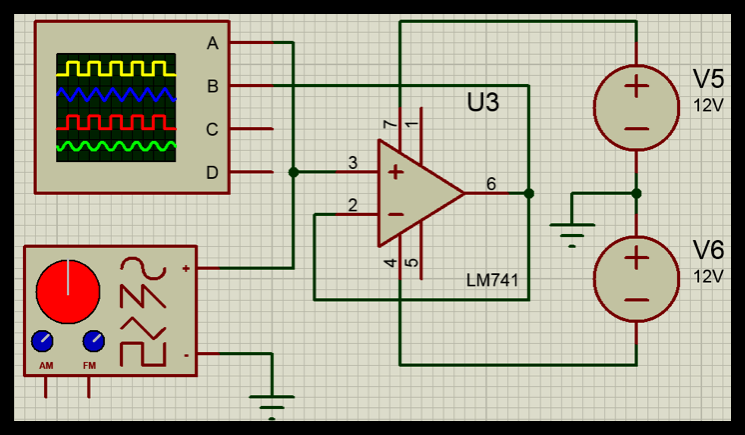
\includegraphics[scale=.6]{s3.png}
\centering \linebreak \linebreak Figure 4.1.2: 9.1 V Zener diode simulation.
\end{figure}
\end{enumerate}

\begin{center}
\begin{tabular}[.5cm]{ c c }
\toprule
Source Voltage & Voltage in $R_{L}$ \\
\midrule
3.0 V & 2.26 V \\
\cmidrule{1-2}
4.0 V & 3.01 V \\
\cmidrule{1-2}
5.0 V & 3.76 V \\
\cmidrule{1-2}
6.0 V & 4.51 V \\
\cmidrule{1-2}
7.0 V & 5.27 V \\
\cmidrule{1-2}
8.0 V & 6.02 V \\
\cmidrule{1-2}
9.0 V & 6.77 V \\
\cmidrule{1-2}
10.0 V & 7.52 V \\
\cmidrule{1-2}
11.0 V & 8.28 V \\
\cmidrule{1-2}
12.0 V & 9.01 V \\
\cmidrule{1-2}
13.0 V & 9.23 V \\
\cmidrule{1-2}
14.0 V & 9.40 V \\
\cmidrule{1-2}
15.0 V & 9.55 V \\
\bottomrule
\end{tabular}
\end{center}
\end{tasks}

\pagebreak